\documentclass[12pt]{article}
\usepackage{graphicx}
\usepackage{xcolor}
\usepackage{amsthm}
\usepackage[hidelinks]{hyperref}

\title{Future of Life}
\author{Dylan Ang}
\date{\today}

\newtheorem*{definition}{Definition}

\begin{document}

\maketitle

\tableofcontents

\section{Diversity}

\subsection{Levels of Diversity}

\paragraph{Genetic Diversity}
Genetic diversity is the total number of genetic characteristics in the genetic makeup of a species, it ranges widely from the number of species to differences within species and can be attributed to the span of survival for a species.

\paragraph{Species Diversity}
Species diversity is defined as the number of species and abundance of each species that live in a particular location. The number of species that live in a certain location is called species richness.

\paragraph{Ecosystem Diversity}
Ecosystem diversity deals with the variations in ecosystems within a geographical location and its overall impact on human existence and the environment. Ecosystem diversity addresses the combined characteristics of biotic properties (biodiversity) and abiotic properties (geodiversity).

\subsection{Protecting Endangered Species}

\begin{itemize}
    \item State Level: California's Species of Special Concern
    \item Federal Level: Endangered Species Act of 1973
    \item International Level: CITES and IUCN
\end{itemize}

\paragraph{World Heritage Sites}
Important cultural or environmental sites that are protected by UNESCO.

\paragraph{The Extinction Vortex in Figure \ref{vortex}}
Representation of how species go extinct over time. Inherent problems with small populations lead to even smaller populations. 

\begin{figure}[tph]
    \centering
    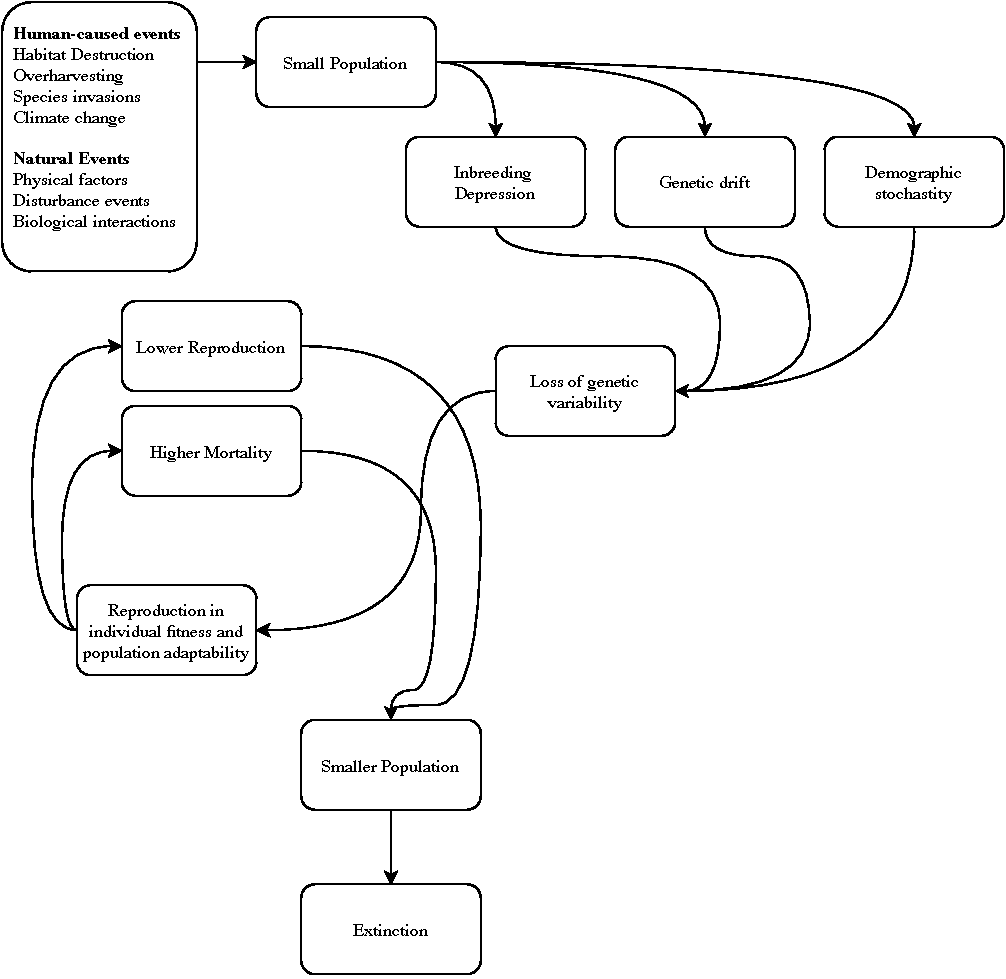
\includegraphics[width=5in]{vortex.pdf}
    \caption{The extinction vortex} \label{vortex}
\end{figure}

\subsection{Approaches to Conservation}

\subsubsection{Small Population Approach}

The small population approach studies the processes that cause extinction once population sizes have been reduced, such as the extinction vortex. This relates to the ideas of the minimum viable population and the effective population size.

\begin{definition}
    The \textbf{minimum viable population} is a lower bound on the population of a species, such that it can survive in the wild.
\end{definition}

\begin{definition}
    The \textbf{effective population size} is the number of individuals that an idealised population would need to have in order for some specified quantity of interest to be the same in the idealised population as in the real population. Takes into account different factors such as breeding population size and genetic diversity.
\end{definition}

\subsubsection{Declining Population Approach}

The declining population approach focuses on threatened and endangered populations that show a downward trend, even if the population is above minimum viable population. This approach gives you a broader picture of ecosystem health, and helps you identify and counteract threats at an earlier stage.

\subsection{How do we allocate resources to conservation?}

Should we spend more resources on \textit{Bufonidae} or \textit{Rheobatrachidae}? Or something in the middle like \textit{Ranidae}. Remember that: 
\begin{itemize}
    \item \textit{Bufonidae} had a large number of species experiencing decline that represented a small portion of the overall group.
    \item \textit{Rheobatrachidae} had a small number of species experiencing decline that represented the entire diversity of that group.
    \item \textit{Ranidae} are in the middle. There are a middling number of species in decline that represent a relatively small portion of the group.
\end{itemize}

There is no single correct answer, but often we want to put our resources into groups that have a higher likelihood of success, rather than wasting money on a lost cause.

\section{Threats and Solutions}

\subsection{Threats to Biodiversity}
\begin{itemize}
    \item Habitat Loss and Alteration
    \item Climate Change
    \item Over-exploitation
    \item Invasive Species
    \item Pollution
\end{itemize}

\subsection{More Details}

\paragraph{Habitat Loss and Alteration}
Habitat loss is the process by which a natural habitat becomes incapable of supporting its native species. The organisms that previously inhabited the site are displaced or dead, thereby reducing biodiversity and species abundance.

\paragraph{Effects of Fragmentation}
In addition to loss of habitat, the process of habitat fragmentation results in three other effects: increase in number of patches, decrease in patch sizes, and increase in isolation of patches. Fragmented habitats have lower species diversity.

\paragraph{Fragmentation and Conservation}
The Monarch Butterfly Biosphere Reserve features intentionally connected fragments to increase species diversity. Since fragmentation harms environments, wildlife corridors can help prevent fragmentation by allowing animals to pass over roads. 

\paragraph{Over-Exploitation}
Overexploitation means harvesting species from the wild at rates faster than natural populations can recover. Overfishing and overhunting are both types of overexploitation. Currently, about a third of the world's endangered vertebrates are threatened by overexploitation.

\paragraph{Pollution: Superfund}
Superfund is a law that was passed in 1980: the goal was to identify and clean up toxic waste sites. Since 1980, 392 sites have been delisted. 

\paragraph{COVID and Conservation}
Some animals benefitted from COVID:
\begin{itemize}
    \item Less urban disturbance $\Rightarrow$ urban population of porcupines increased.
    \item Less people on beaches $\Rightarrow$ Shore birds population increased.
    \item Higher fertility rates in birds.
    \item Higher diurnal(daytime) activity in rabbits.
\end{itemize} 

There were some negatives; mainly that conservation and restoration activities like invasive species management or endangered species support activities were halted during quarantine. In addition, there is less enforcement of rules, so people may steal/disturb endangered species more. 

\section{The Sixth Extinction}

There have been 5 major extinctions: we covered them in the history of life lecture. This section discusses whether we are currently in a sixth major extinction. In order to satisfy the criteria, we need to have extinction rates higher than a certain ``background rate''. 

\begin{figure}[tph]
    \centering
    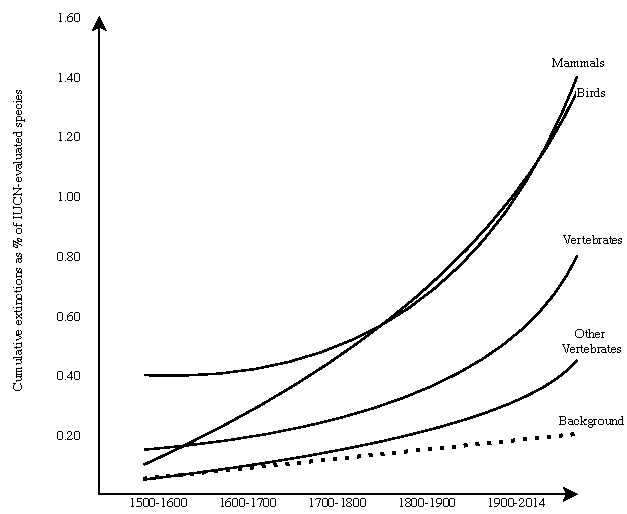
\includegraphics[width=5in]{extinction.pdf}
    \caption{Earth's sixth mass extinction} \label{extinction}
\end{figure}

In order to be considered a mass extinction, we need at least 75\% of species to go extinct. If currently threatened species go extinct, we still will not reach mass extinction percentages: we are around 65\% for some groups.

\paragraph{The True Silent Spring}
Since 1970, the population size of birds has decreased by about 3 million birds. Nature is more silent now since the birbs have gone quiet.

\paragraph{The Half-Earth Project}
Goal to have 50\% of Earth's area to be protected.

\begin{itemize}
    \item If we have 100\% habitat loss, we can retain 0\% species.
    \item If we have 90\% habitat loss, we can retain 50\% species.
    \item If we have 50\% habitat loss, we can retain 85\% species.
\end{itemize}

\end{document}